\chapter{KHẢO SÁT TÍNH ỔN ĐỊNH CỦA HỆ THỐNG}
    Ta có hàm truyền đã tìm được ở trên là:
    \[
        G(s) = \frac{4.85}{s^2 + 53.51}
    \]
    Hệ vòng kín với phản hồi là: 
    \[
        T(s) = \frac{G(s)}{1+G(s)} 
    \]
    Phương trình đặc tính:
    \begin{align*}
        &1 + G(s) = 0 \\
        &\Leftrightarrow 1 + \frac{4.85}{s^2 + 53.51} = 0 \\
        &\Leftrightarrow s^2 + 58.36 = 0
    \end{align*}
    $\Leftarrow$ Hệ không ổn định do hệ số của $s^1$ là 0. 
    \section{Biểu đồ Bode}
    \[
        G(s) = \frac{4.85}{s^2 + 53.51}
    \]
    Phân tích:
    \begin{itemize}
        \item 1 khâu khuếch đại: K = 4.85.
        \item 1 khâu dao động bậc 2.
    \end{itemize}
    Tần số cộng hưởng: 
    \[
        \omega_n = \sqrt{53.51} = 7.315 (rad/s)
    \]
    Đặc tính tần số:
    \[
        G_1(j\omega) = \frac{4.85}{-\omega^2 + 53.51}
    \]
    \textbf{Biên độ:}
    \[
        M(\omega) = \abs{G(j\omega)} = \frac{4.85}{\abs{-\omega^2 + 53.51}}
    \]
    \[
        \Rightarrow L(\omega) = 20log(M(\omega)) = 20log(4.85) - 20log(\abs{-\omega^2 + 53.51})
    \]
    \begin{itemize}
        \item Khi $0<\omega<7.315$: biên độ tăng từ -20.85dB đến $+\infty$
        \item Với $\omega > 7.315$: 
    \end{itemize}
    \begin{align*}
        &20log(4.85) - 20log(\abs{-\omega^2 + 53.51}) \approx 20log(4.85) - 20log(\omega^2) \\
        &= 20log(4.85) - 40log(\omega) \\
        &\Rightarrow \text{Độ dốc giảm: } -40dB/decade \\
        &\Rightarrow \text{Với } \omega > 7.315: \text{ biên độ giảm từ } +\infty \text{ về } -\infty
    \end{align*}
    \textbf{Pha:}
    \[
        \angle G(j\omega) =
        \begin{cases}
            0 \quad ;\quad \omega < 7{,}315 \\
            -180^\circ \quad ;\quad \omega > 7{,}315 \\
            \text{Pha nhảy từ 0 xuống } -180^\circ \text{ tại } \omega = 7.315
        \end{cases}
    \]
    \begin{figure}[H]
        \centering
        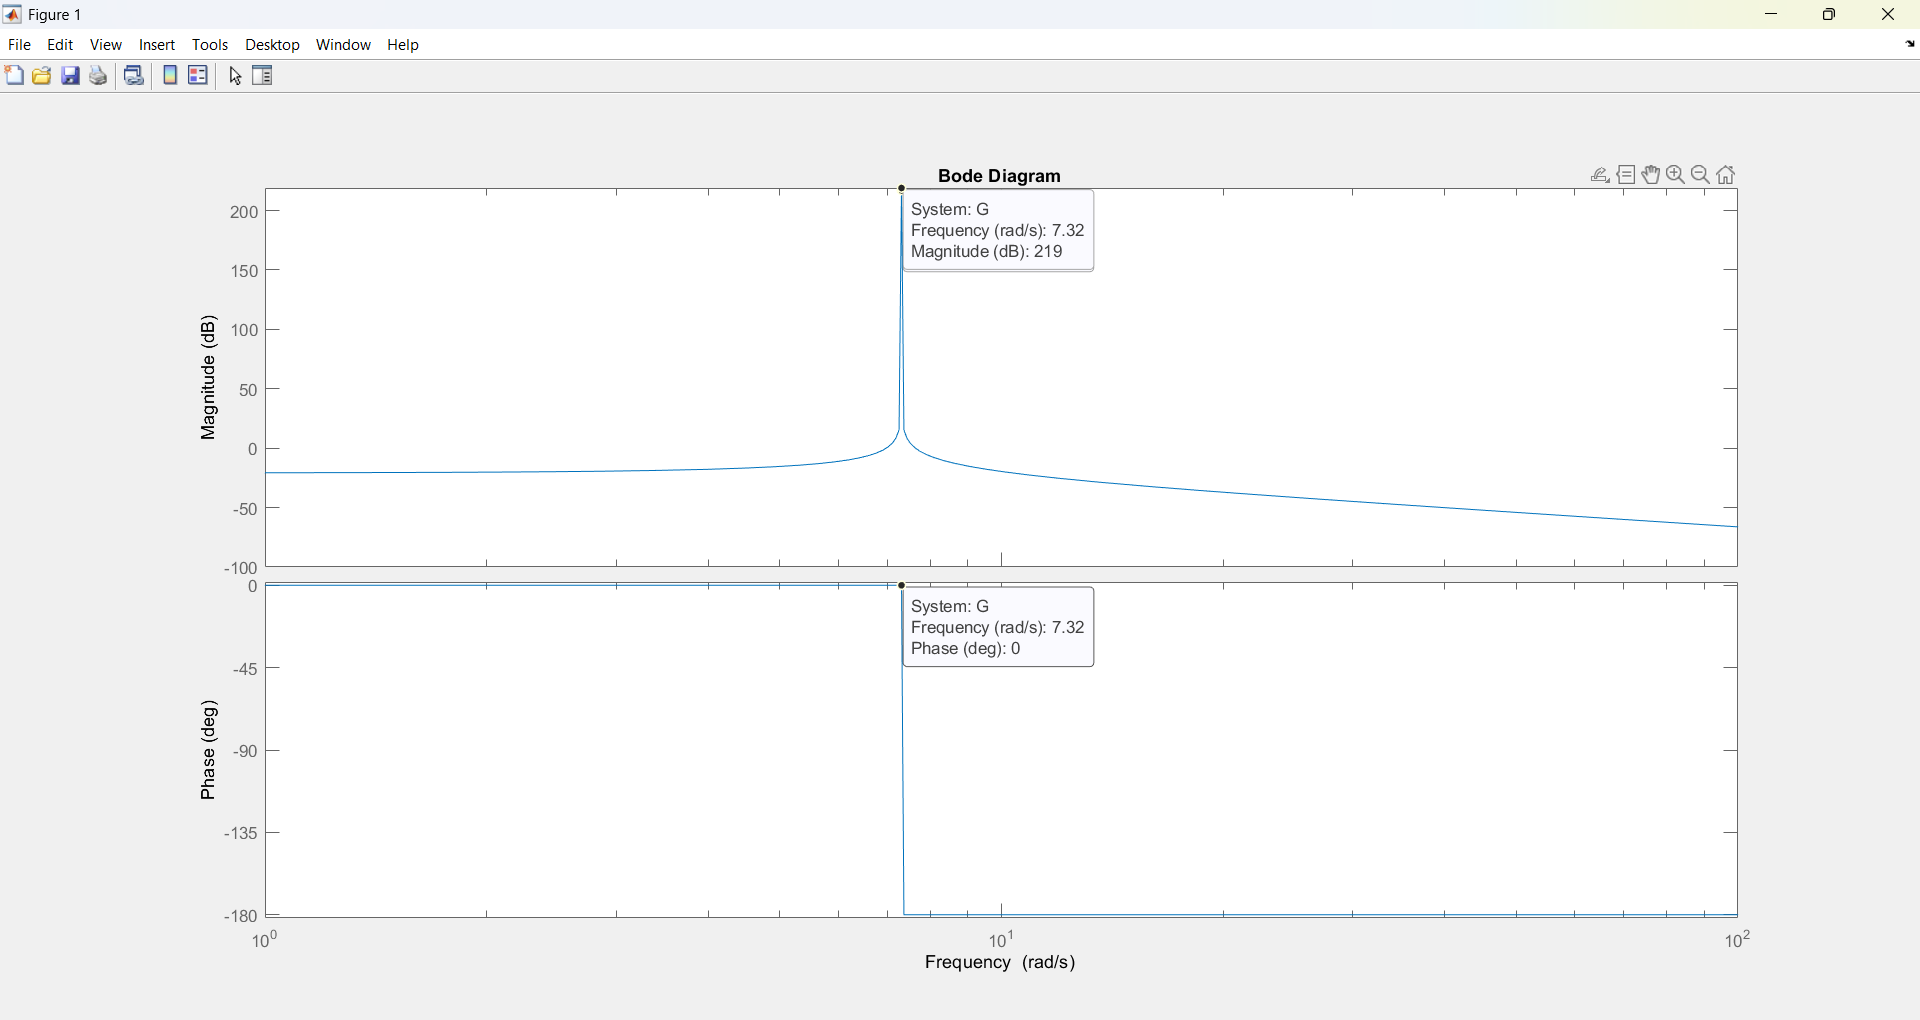
\includegraphics[width=1\textwidth]{pictures/bode.png}
    \end{figure}
    Nhận xét:
    \begin{itemize}
        \item Hệ thống vòng hở: G(s) có các cực trên trục ảo $s=+-7.315$ nên hệ thống ổn định biên. Đồ thị Bode cho thấy biên độ đạt đỉnh tại $\omega=7.315$ và pha nhảy xuống là $-180^\circ$. Điều này xác nhận hệ thống dao động không suy giảm.
        \item Từ độ thị ta có thể thấy độ dữ trữ pha $G_M < 0 dB$ nên đã vi phạm tiêu chuẩn ổn định của biểu đồ Bode $\Rightarrow$ Hệ chưa ổn định. 
    \end{itemize}
